\documentclass{beamer}

% Theme and color scheme
\usetheme{Madrid}
\usecolortheme{whale}
\usepackage{xcolor}
\usepackage{etoolbox}

% Packages
\usepackage{graphicx}
\usepackage{hyperref}
\usepackage[backend=biber, sorting=none]{biblatex}
\addbibresource{refs.bib}
\DeclareFieldFormat*{title}{#1}
\DeclareFieldFormat*{url}{\newline\url{#1}\nopunct}
\DeclareFieldFormat{labelnumberwidth}{#1\adddot}
\setlength{\biblabelsep}{5pt}
\renewcommand*{\bibfont}{\tiny}
\usepackage{ragged2e}

\newcommand{\biburl}[2][]{%
  \newline - \ifstrempty{#1}{}{\textcolor{cyan}{#1: }}\url{#2}\nopunct
}

% Title and author information
\title{ChatGPT Survey}
\subtitle{A Programmer's Perspective}
\author{Yu Zehan}
\institute{Intel FLEX}
\date{\today}

\begin{document}

% Title slide
\begin{frame}
  \titlepage
\end{frame}

% Table of contents
\begin{frame}{Outline}
  \tableofcontents
\end{frame}

\section{Philosophies and methodologies}
\begin{frame}{Philosophies and Methodologies}
  \begin{itemize}
    \item Philosophies: Two Views
    \begin{itemize}
      \item Lifecycle of a Python Project
    \end{itemize}
    \item Methodologies: Master ChatGPT
  \end{itemize}
\end{frame}

\section{Life cycle of program development}
\begin{frame}{Lifecycle of a Python project}
  \begin{enumerate}
  \item Requirements analysis
  \item Design and architecture
  \item Environment setup
  \item Develop
  \item Test
  \item Code review
  \item Debug and optimize
  \item Deploy and maintain
  \item Document
\end{enumerate}
\end{frame}

\begin{frame}{TikZ Test}
  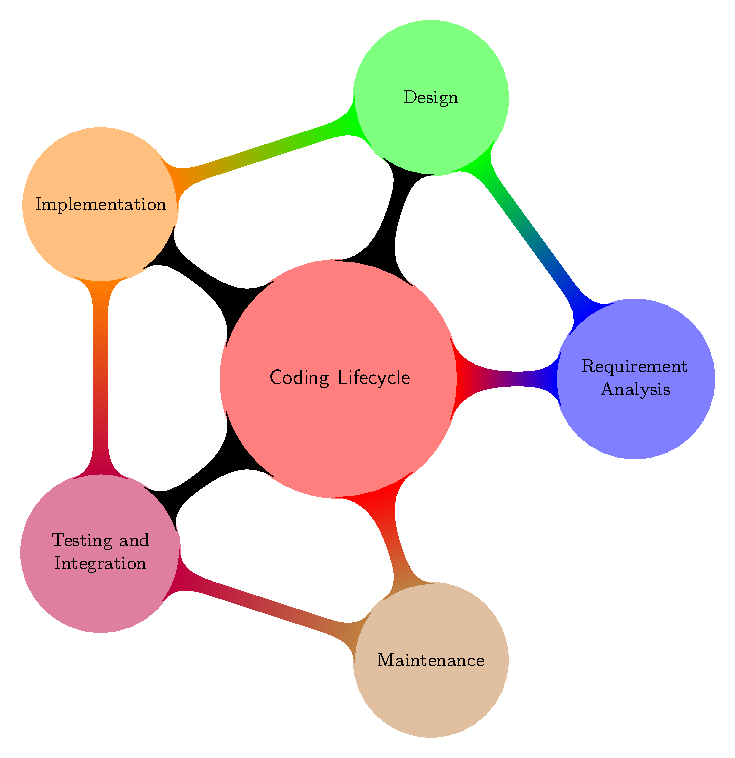
\includegraphics[width=\textwidth,height=0.8\textheight,keepaspectratio]{tikz-code-lifecycle.pdf}
\end{frame}

\begin{frame}{Outline}
  \begin{itemize}
    \item Prototype and Example
    \item Debug
    \item Code Review: Styles, Documentation, Comments
    \item Resources and Knowledge Database
    \item Roadmap
    \item Project plan
    \item Tools, utils, libraries and softwares
    \item Code \cite{coding-prompts}
  \end{itemize}
\end{frame}

\section{Prototype}
\begin{frame}{Prototype}
\end{frame}

\section{Debug}
\begin{frame}{Debug}
\end{frame}

% 行动指南(instructions)、事实依据(facts)、思想纲领(policies)

\section{References}
\begin{frame}[t,allowframebreaks]{References}
  \nocite{*}
  \RaggedRight
  \printbibliography
\end{frame}


% Closing slide
\begin{frame}{FAQ}

\end{frame}

\end{document}
